%%%%%%%%%%%%%%%%%%%%%%%%%%%%%%%%%%%%%%%%%%%%%%%%%%%%%%%%%%%%%%%%%%%%%%%%%%%%%%%%
%%%%%%%%%%%%%%%%%%%%%%%%%%%%%%%%%%%%%%%%%%%%%%%%%%%%%%%%%%%%%%%%%%%%%%%%%%%%%%%%
%\documentclass[addpoints,12pt,solution]{exam}
\documentclass[preprint,12pt]{elsarticle}
%% Use the option review to obtain double line spacing

%% Use the options 1p,twocolumn; 3p; 3p,twocolumn; 5p; or 5p,twocolumn
%% for a journal layout:
%% \documentclass[final,1p,times]{elsarticle}
%% \documentclass[final,1p,times,twocolumn]{elsarticle}
%% \documentclass[final,3p,times]{elsarticle}
%% \documentclass[final,3p,times,twocolumn]{elsarticle}
%% \documentclass[final,5p,times]{elsarticle}
%% \documentclass[final,5p,times,twocolumn]{elsarticle}

%% The graphicx package provides the includegraphics command.
\usepackage{graphicx}
%% The amssymb package provides various useful mathematical symbols
\usepackage{amssymb}
\usepackage{amsmath}
\usepackage{breqn}
\usepackage{chemfig}
\usepackage{csvsimple}
%% The amsthm package provides extended theorem environments
%% \usepackage{amsthm}

%% The lineno packages adds line numbers. Start line numbering with
%% \begin{linenumbers}, end it with \end{linenumbers}. Or switch it on
%% for the whole article with \linenumbers after \end{frontmatter}.
\usepackage{lineno}
\usepackage{natbib}
\usepackage{hyperref}
% \usepackage[top=0.75in, bottom=0.75in, left=0.55in, right=0.85in]{geometry}
\usepackage{graphicx}
\usepackage{url}
\usepackage{palatino}
\usepackage{tabularx}
\usepackage{graphicx}
\usepackage{multicol}
\usepackage{graphicx}
\usepackage{amssymb}
\usepackage{float}
\usepackage{amsmath}
\usepackage{rotating}
\usepackage{subfigure}
\usepackage{multirow}
\usepackage{mathrsfs}
\usepackage{xfrac}
\usepackage[font=small,skip=0pt]{caption}
%\usepackage[numbers,sort&compress]{natbib}
%\usepackage{hyperref}
\usepackage{pgf,tikz}
\usetikzlibrary{shapes,arrows,chains}
\usetikzlibrary[calc]
\usepackage{graphicx}
\graphicspath{ {./images/} }

\usepackage{geometry}
\geometry{lmargin=1in,rmargin=1in,tmargin=1in,bmargin=1in}
\usepackage{lipsum}
%\pagestyle{empty}
\usepackage{natbib}
\pagenumbering{arabic}
%\usepackage[T1]{fontenc}
\usepackage{setspace}
\usepackage{mathptmx}
\usepackage{t1enc}
%\usepackage{xkeyval}
%\usepackage{chemformula}
%\usepackage{array}
%\usepackage{booktabs}
%\usepackage{hypdoc}
%\usepackage{listings}
%\usepackage{lmodern}
%\usepackage{mathpazo}
%\usepackage{microtype}
\usepackage{graphicx}
\usepackage{amssymb}
\usepackage{float}
\usepackage{amsmath}
\usepackage{rotating}
\usepackage{subfigure}
\usepackage{multirow}
\usepackage{xfrac}
\usepackage[font=small,skip=0pt]{caption}
%\usepackage[numbers,sort&compress]{natbib}
%\usepackage{hyperref}
\usepackage{pgf,tikz}
\usetikzlibrary{shapes,arrows,chains}
\usetikzlibrary[calc]
\usepackage{graphicx}
\usepackage{geometry}
\geometry{lmargin=1in,rmargin=1in,tmargin=1in,bmargin=1in}
\usepackage{lipsum}
%\pagestyle{empty}
\usepackage{natbib}
\pagenumbering{arabic}
%\usepackage[T1]{fontenc}
\usepackage{setspace}
\usepackage{mathptmx}
\usepackage{t1enc}
%\usepackage{xkeyval}
%\usepackage{chemformula}
%\usepackage{array}
%\usepackage{booktabs}
%\usepackage{hypdoc}
%\usepackage{listings}
%\usepackage{lmodern}
%\usepackage{mathpazo}
%\usepackage{microtype}
\usepackage{lineno,hyperref}
\usepackage{multirow}
\usepackage{cancel}
\usepackage{url}
\usepackage[norule]{footmisc}
\usepackage[utf8]{inputenc}
\usepackage[english]{babel}
\hypersetup{colorlinks = true,linkcolor = blue,urlcolor = blue}
% \fontfamily{SansSerif}
% \selectfont
% \usepackage[T1]{fontenc}
% \usepackage
%% natbib.sty is loaded by default. However, natbib options can be
%% provided with \biboptions{...} command. Following options are
%% valid:
%%   round  -  round parentheses are used (default)
%%   square -  square brackets are used   [option]
%%   curly  -  curly braces are used      {option}
%%   angle  -  angle brackets are used    <option>
%%   semicolon  -  multiple citations separated by semi-colon
%%   colon  - same as semicolon, an earlier confusion
%%   comma  -  separated by comma
%%   numbers-  selects numerical citations
%%   super  -  numerical citations as superscripts
%%   sort   -  sorts multiple citations according to order in ref. list
%%   sort&compress   -  like sort, but also compresses numerical citations
%%   compress - compresses without sorting
%%
%% \biboptions{comma,round}
% \biboptions{}
\usepackage{caption}
\usepackage{caption}
\usepackage{algorithm} 
\usepackage[noend]{algpseudocode}
\usepackage{amsmath}
\DeclareMathOperator*{\argmin}{argmin}
\DeclareMathOperator*{\argmax}{argmax}
\newcommand*{\argminl}{\argmin\limits}
\newcommand*{\argmaxl}{\argmax\limits}



\begin{document}


\hrule
\vspace{1mm}
\noindent 
\begin{center}
{\Large CS6700 : Reinforcement Learning} \\

{\large Programming Assignment Report-1} \\
{\large Control Algorithms   \hfill }
\end{center}
\vspace{1mm}
\noindent 



%%%%%%%%%%%%%%%%%%%%%%%%%%%%%%%%%%%%%%%%%%%%%%%%%%%%%%%%%%%%%%%%
% Enter name and roll number here
\noindent {\bf Name:} Pragnesh Rana \hfill {\bf Roll number:} ME17S301
%%%%%%%%%%%%%%%%%%%%%%%%%%%%%%%%%%%%%%%%%%%%%%%%%%%%%%%%%%%%%%%%%%
\vspace{2mm}
\hrule

{\small

\begin{itemize}\itemsep0mm
\item Part-A is on Puddle GridWorld
\item Part-B is about Policy Gradient Implementation 
\end{itemize}
}
\hrule
\vspace{3mm}
newpage


%%
%% Following citation commands can be used in the body text:
%% Usage of \cite is as follows:

%%   \cite{key}          ==>>  [#]
%%   \cite[chap. 2]{key} ==>>  [#, chap. 2]
%%   \citet{key}         ==>>  Author [#]

\section{Puddle World:}

 Puddle world has been implemented with different maps. Map-A and Map-B has different terminal states whereas, Map-C has westerly wind blowing which forces the agent to move in east with 0.5 probability. The grid world has puddle in the centre. each state in the world is denoted by different colours. 

Penalty/reward given to the agent varies based on state and transition.  For every transition from one state to another 0 reward is given. In the puddle zone, blue area gives reward of -1 likewise as inside penalty increases. Green and red gives -2, -3 respectively. Puddle world is stochastic in nature. It takes correct action with probability 0.9 where as other action are taken with 0.033 probability equally.Pink shows the terminal state which gives reward of +10 as shown in fig:\ref{fig:puddle}.

\begin{figure}[H]
	\centering  
	\subfigure[Puddle World-A]
	{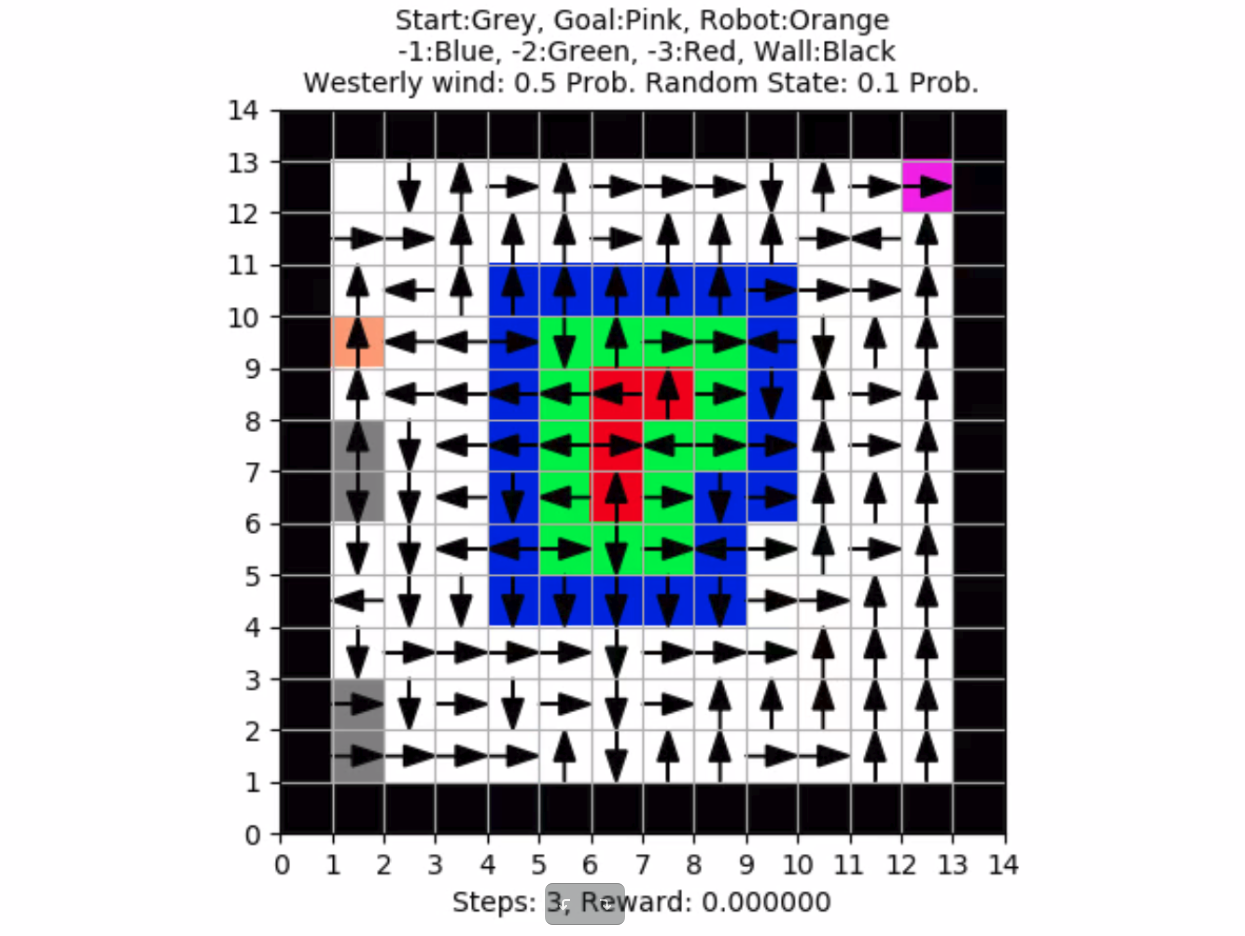
\includegraphics[width=0.35\linewidth]{./Puddle_A.png}}
	\subfigure[Puddle World-B]
	{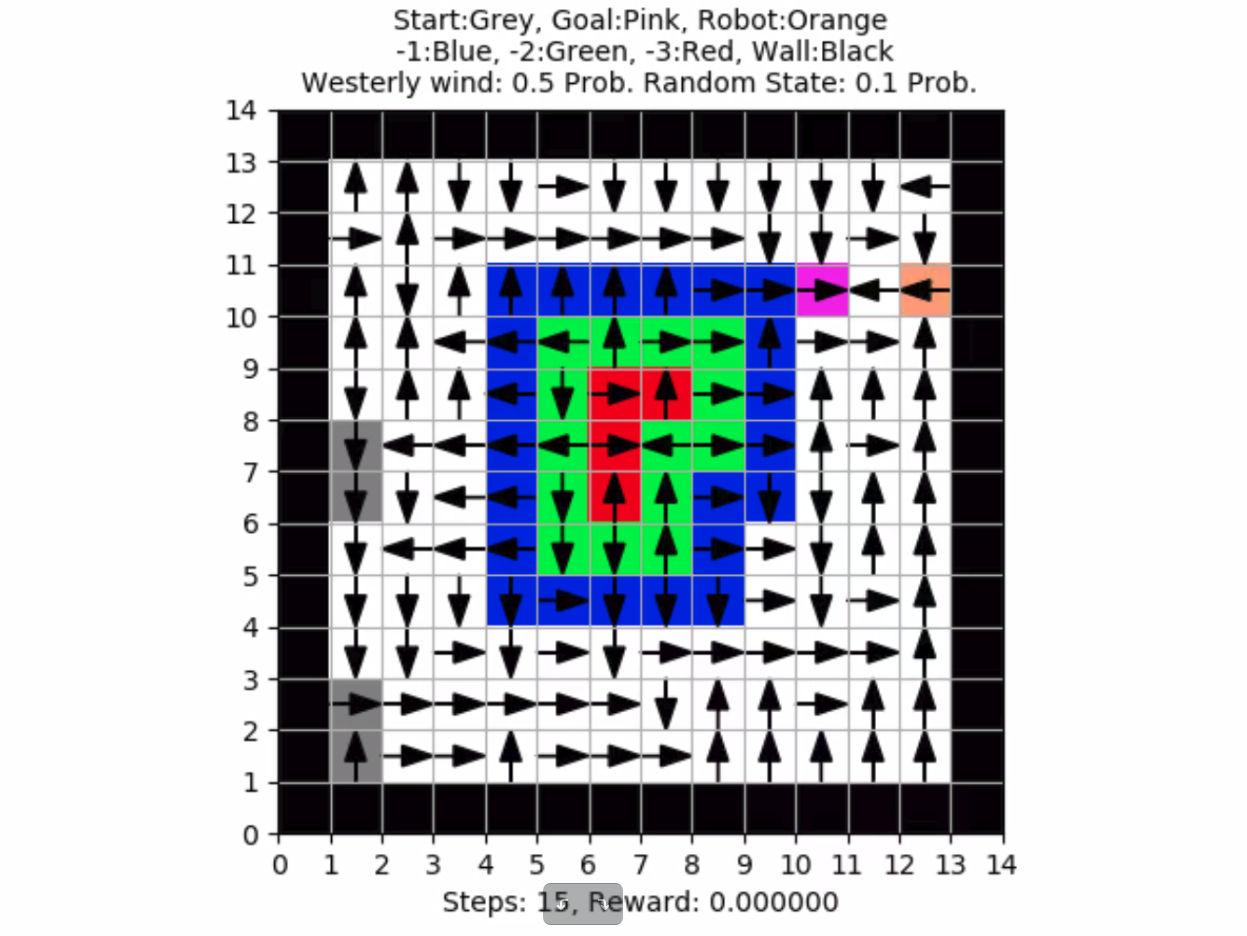
\includegraphics[width=0.35\linewidth]{./Puddle_B.png}}
	\subfigure[Puddle World-C]
	{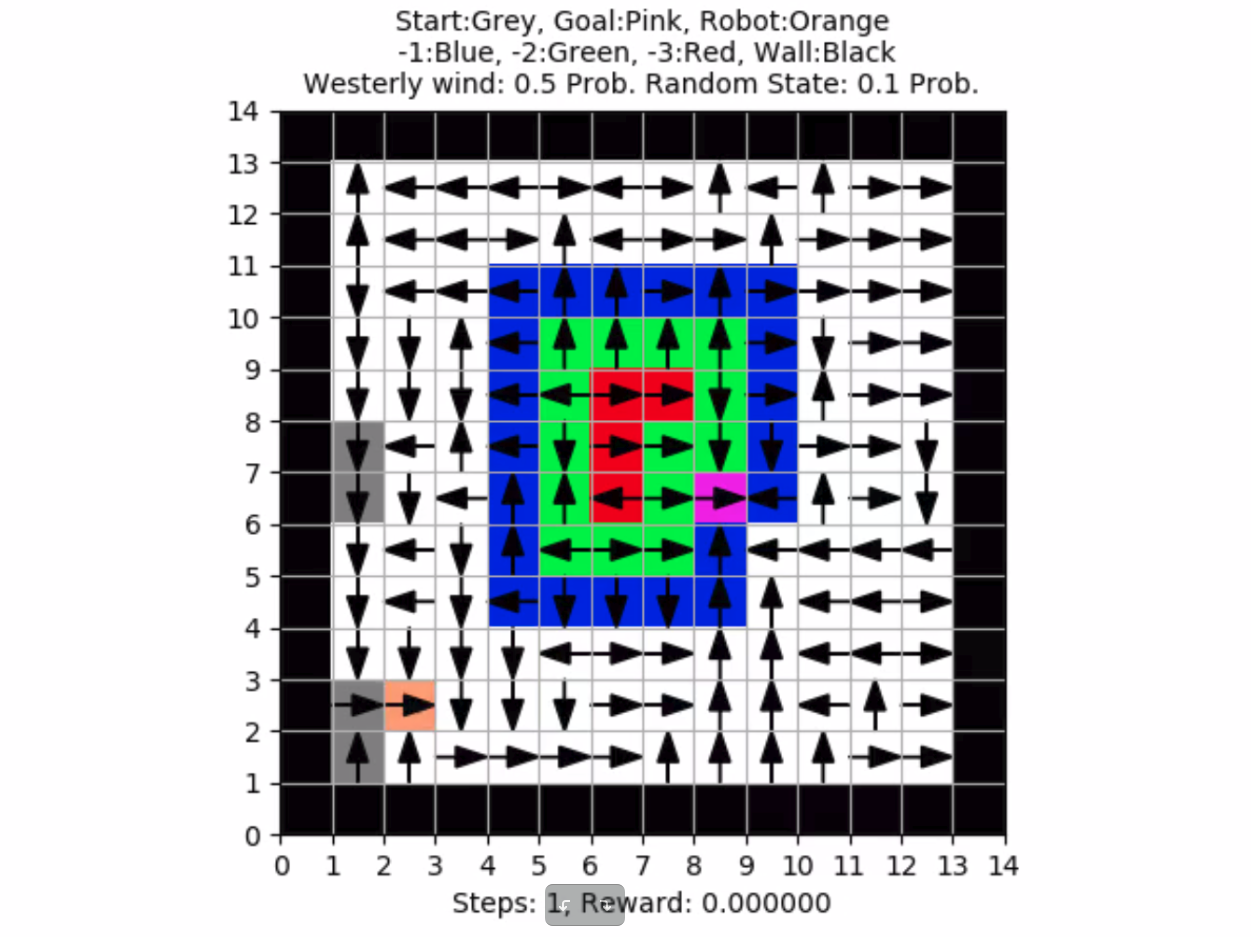
\includegraphics[width=0.35\linewidth]{./Puddle_C.png}}
	\caption{Puddle World with different colour: Grey:Start, Pink:Terminal, Middle:Puddle }
	\label{fig:puddle}
\end{figure}

In Puddle World-C, westerly wind also blowing which forces the agent to move in east direction with probability of 0.5. Suppose agent wanted to go in desired state s' with probability 0.9 and reward will be -1 due to transition but due to wind it may happen that agent may end up in the another state s'' with probability 0.5 and assume such state has higher negative reward then wind misguides the agent.

\subsection{Q-learning:}
The goal is to reach the terminal state with highest possible reward. ran the code for 500 episodes and average steps and return has been computed for 50 runs. 
For each case discount rate $\gamma$ is taken as 0.9, learning rare $\alpha$ is taken as 0.1 and exploration parameter is taken as $\epsilon$= 0.1. 

Epsilon-greedy policy has been used for the exploration. Initially the epsilon was set as 0.1 but as it takes may steps to compute the terminal state. so epsilon value has been boosted to 0.2 . 

\begin{figure}[H]
	\centering  
	\subfigure[Puddle World-A]
	{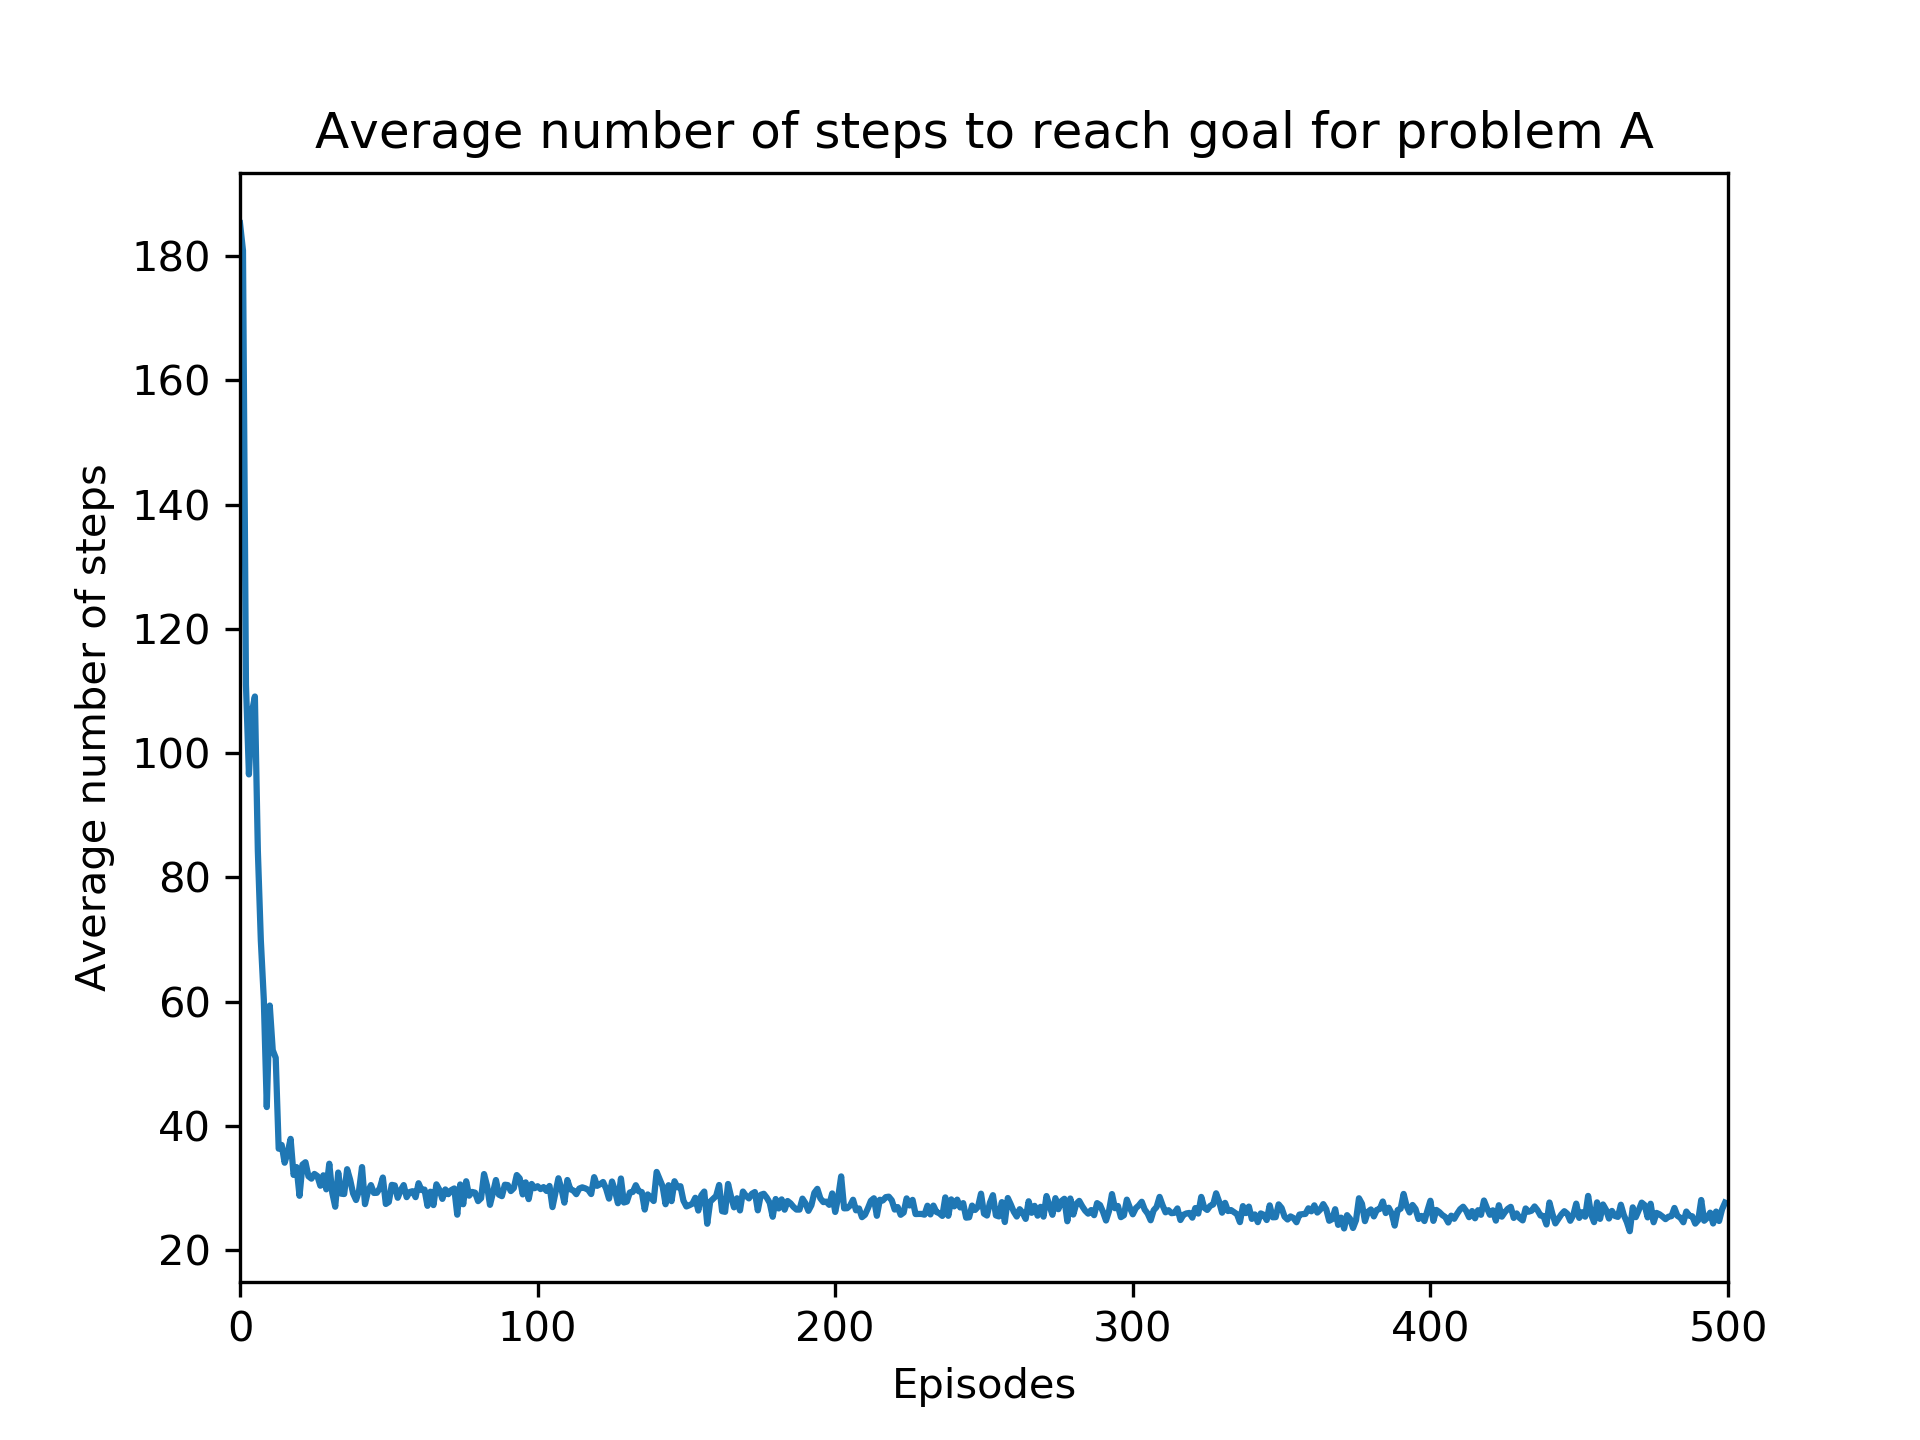
\includegraphics[width=0.43\linewidth]{./QAvg_steps_A500.png}}
	\subfigure[Puddle World-B]
	{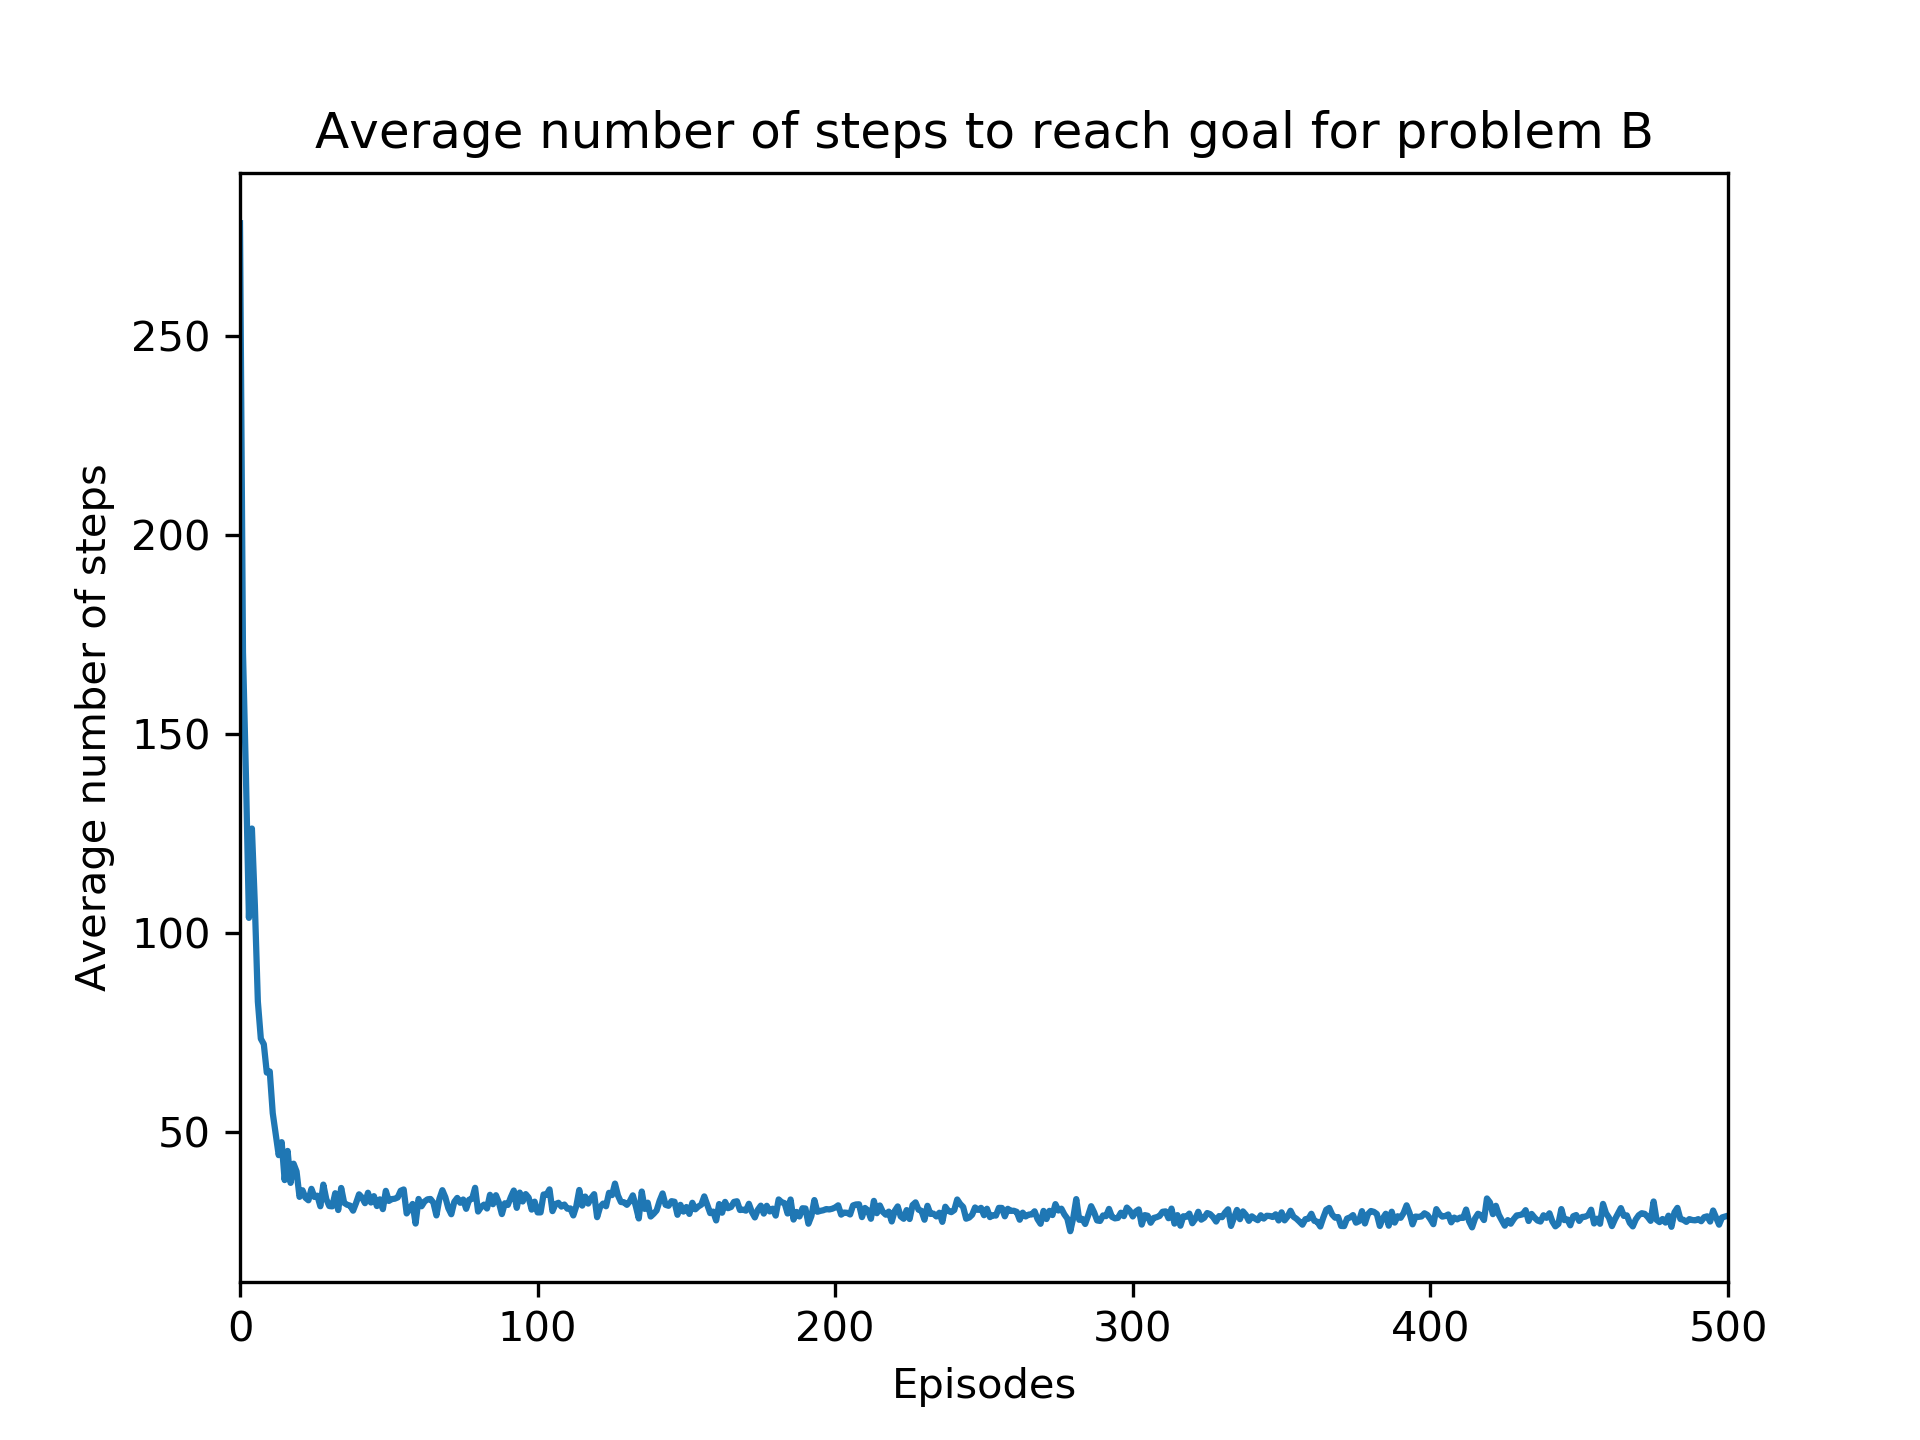
\includegraphics[width=0.43\linewidth]{./QAvg_steps_B500.png}}
	\subfigure[Puddle World-C]
	{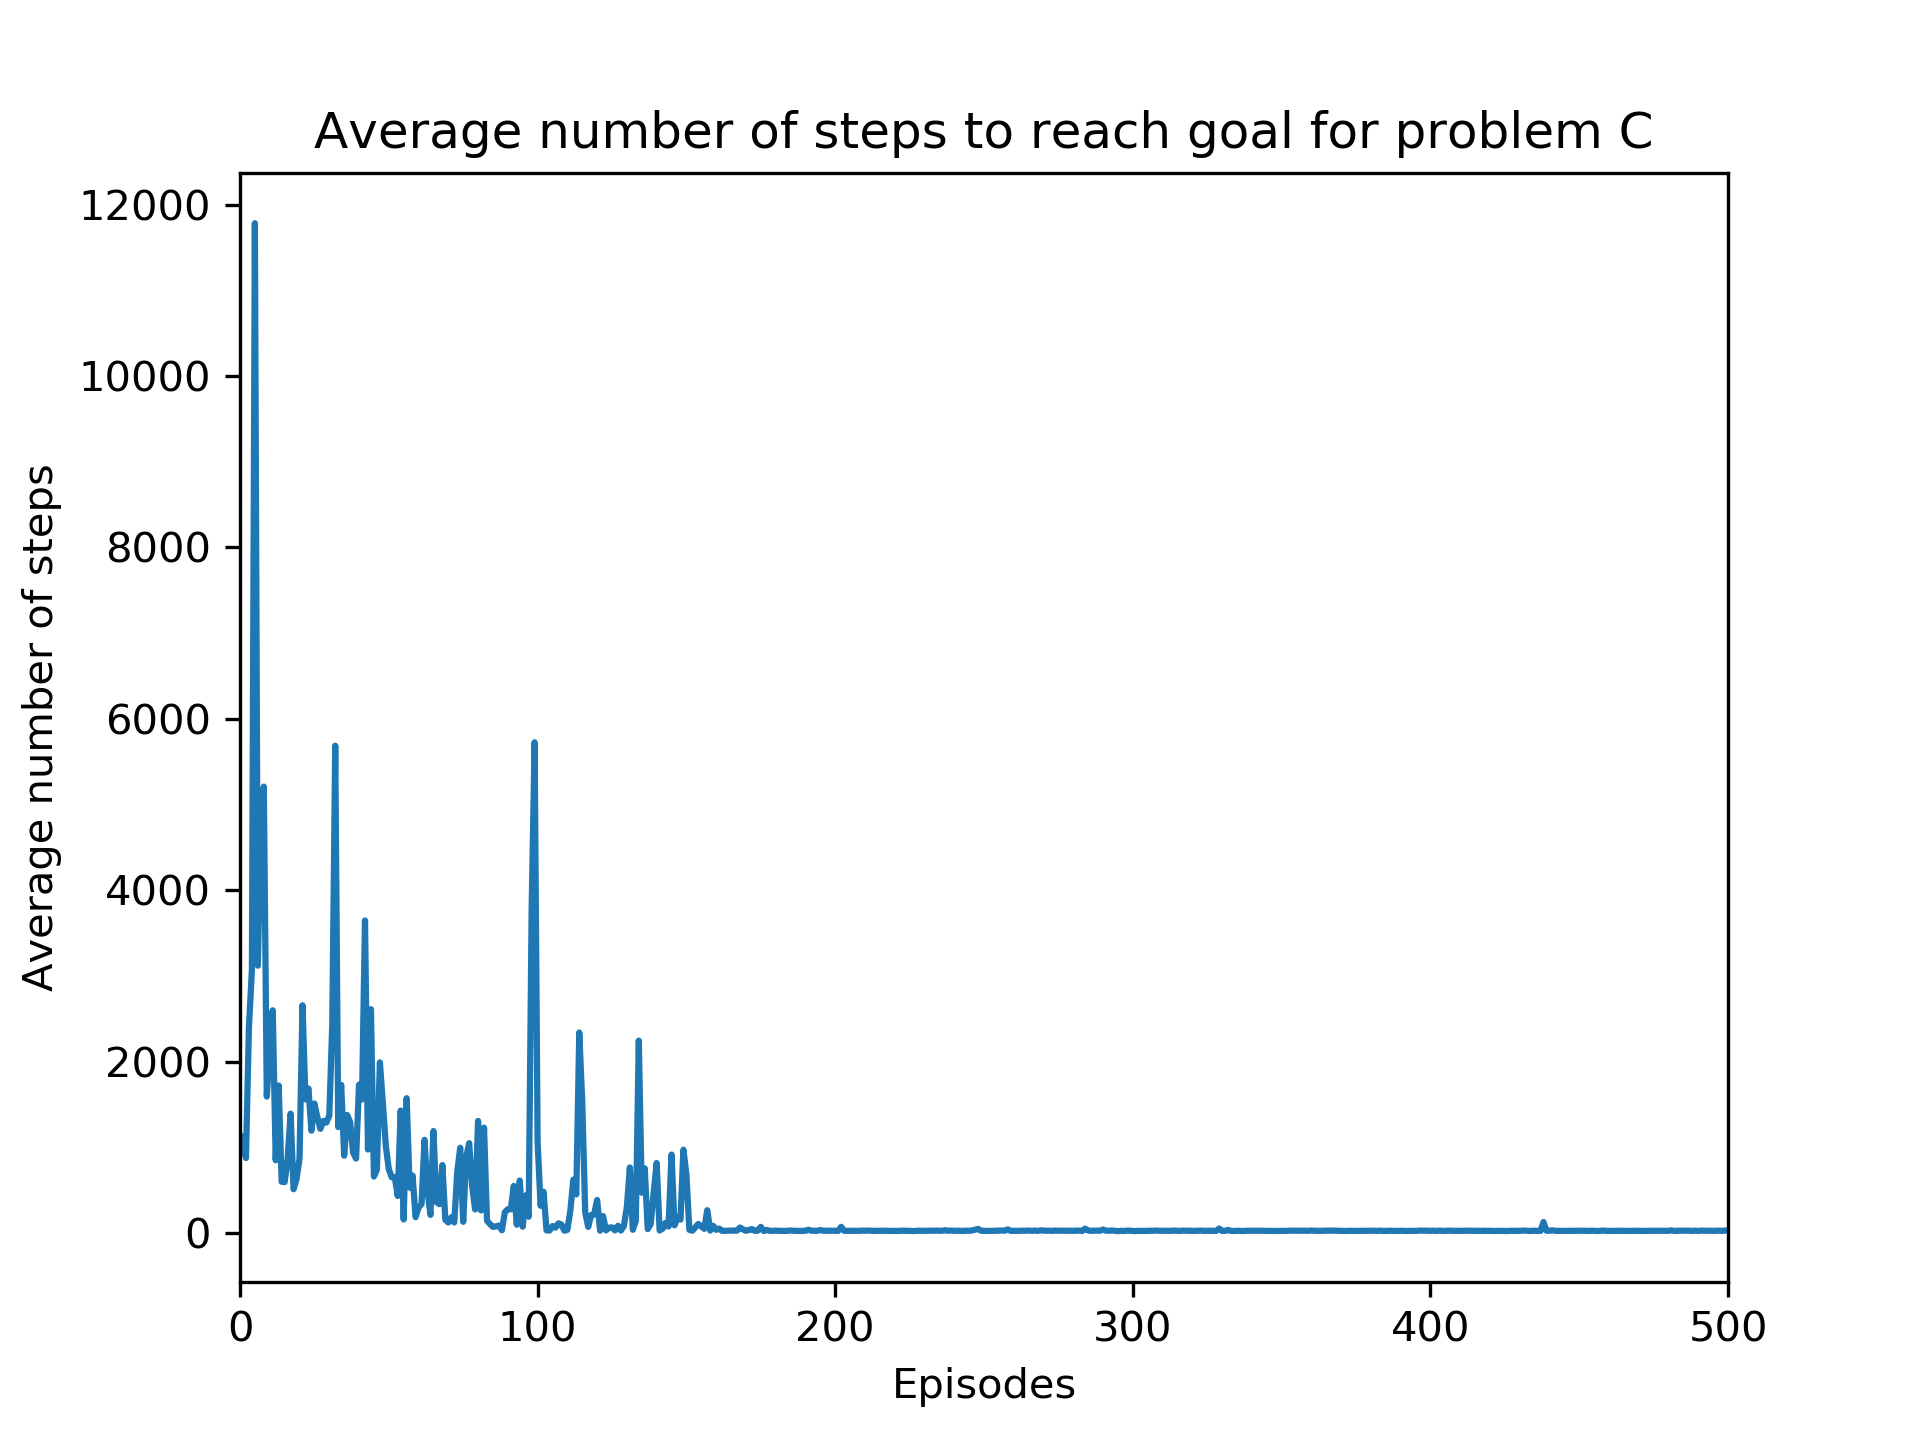
\includegraphics[width=0.43\linewidth]{./QAvg_steps_C500.png}}
	\caption{Average steps taken by the agent in different world}
	\label{fig:stepsQ}
\end{figure}


\begin{figure}[H]
	\centering  
	\subfigure[Puddle World-A]
	{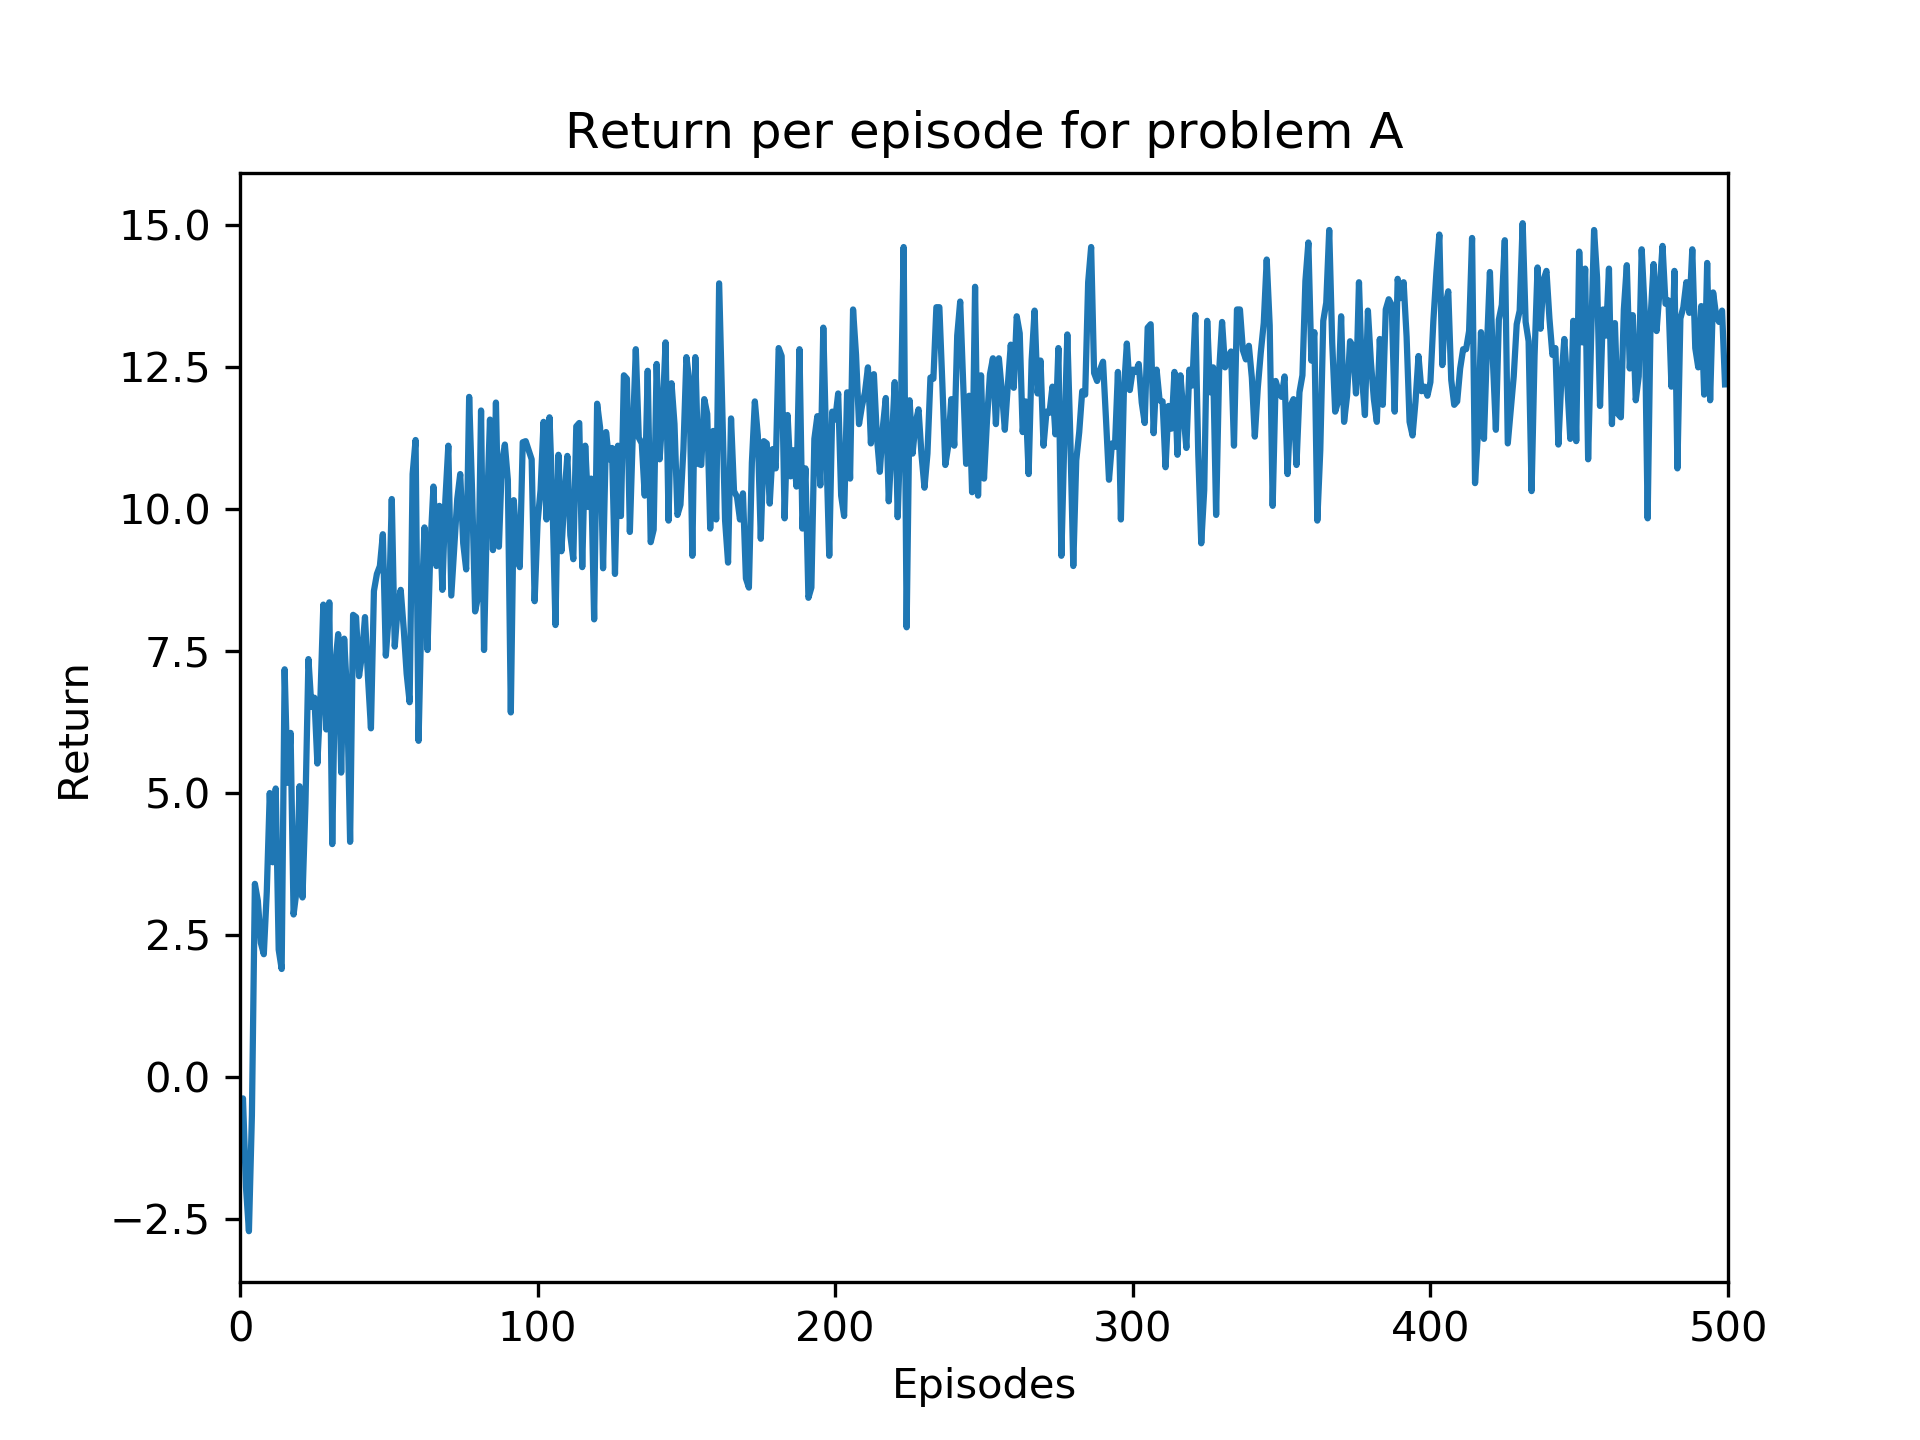
\includegraphics[width=0.4\linewidth]{./QReturn_A500.png}}
	\subfigure[Puddle World-B]
	{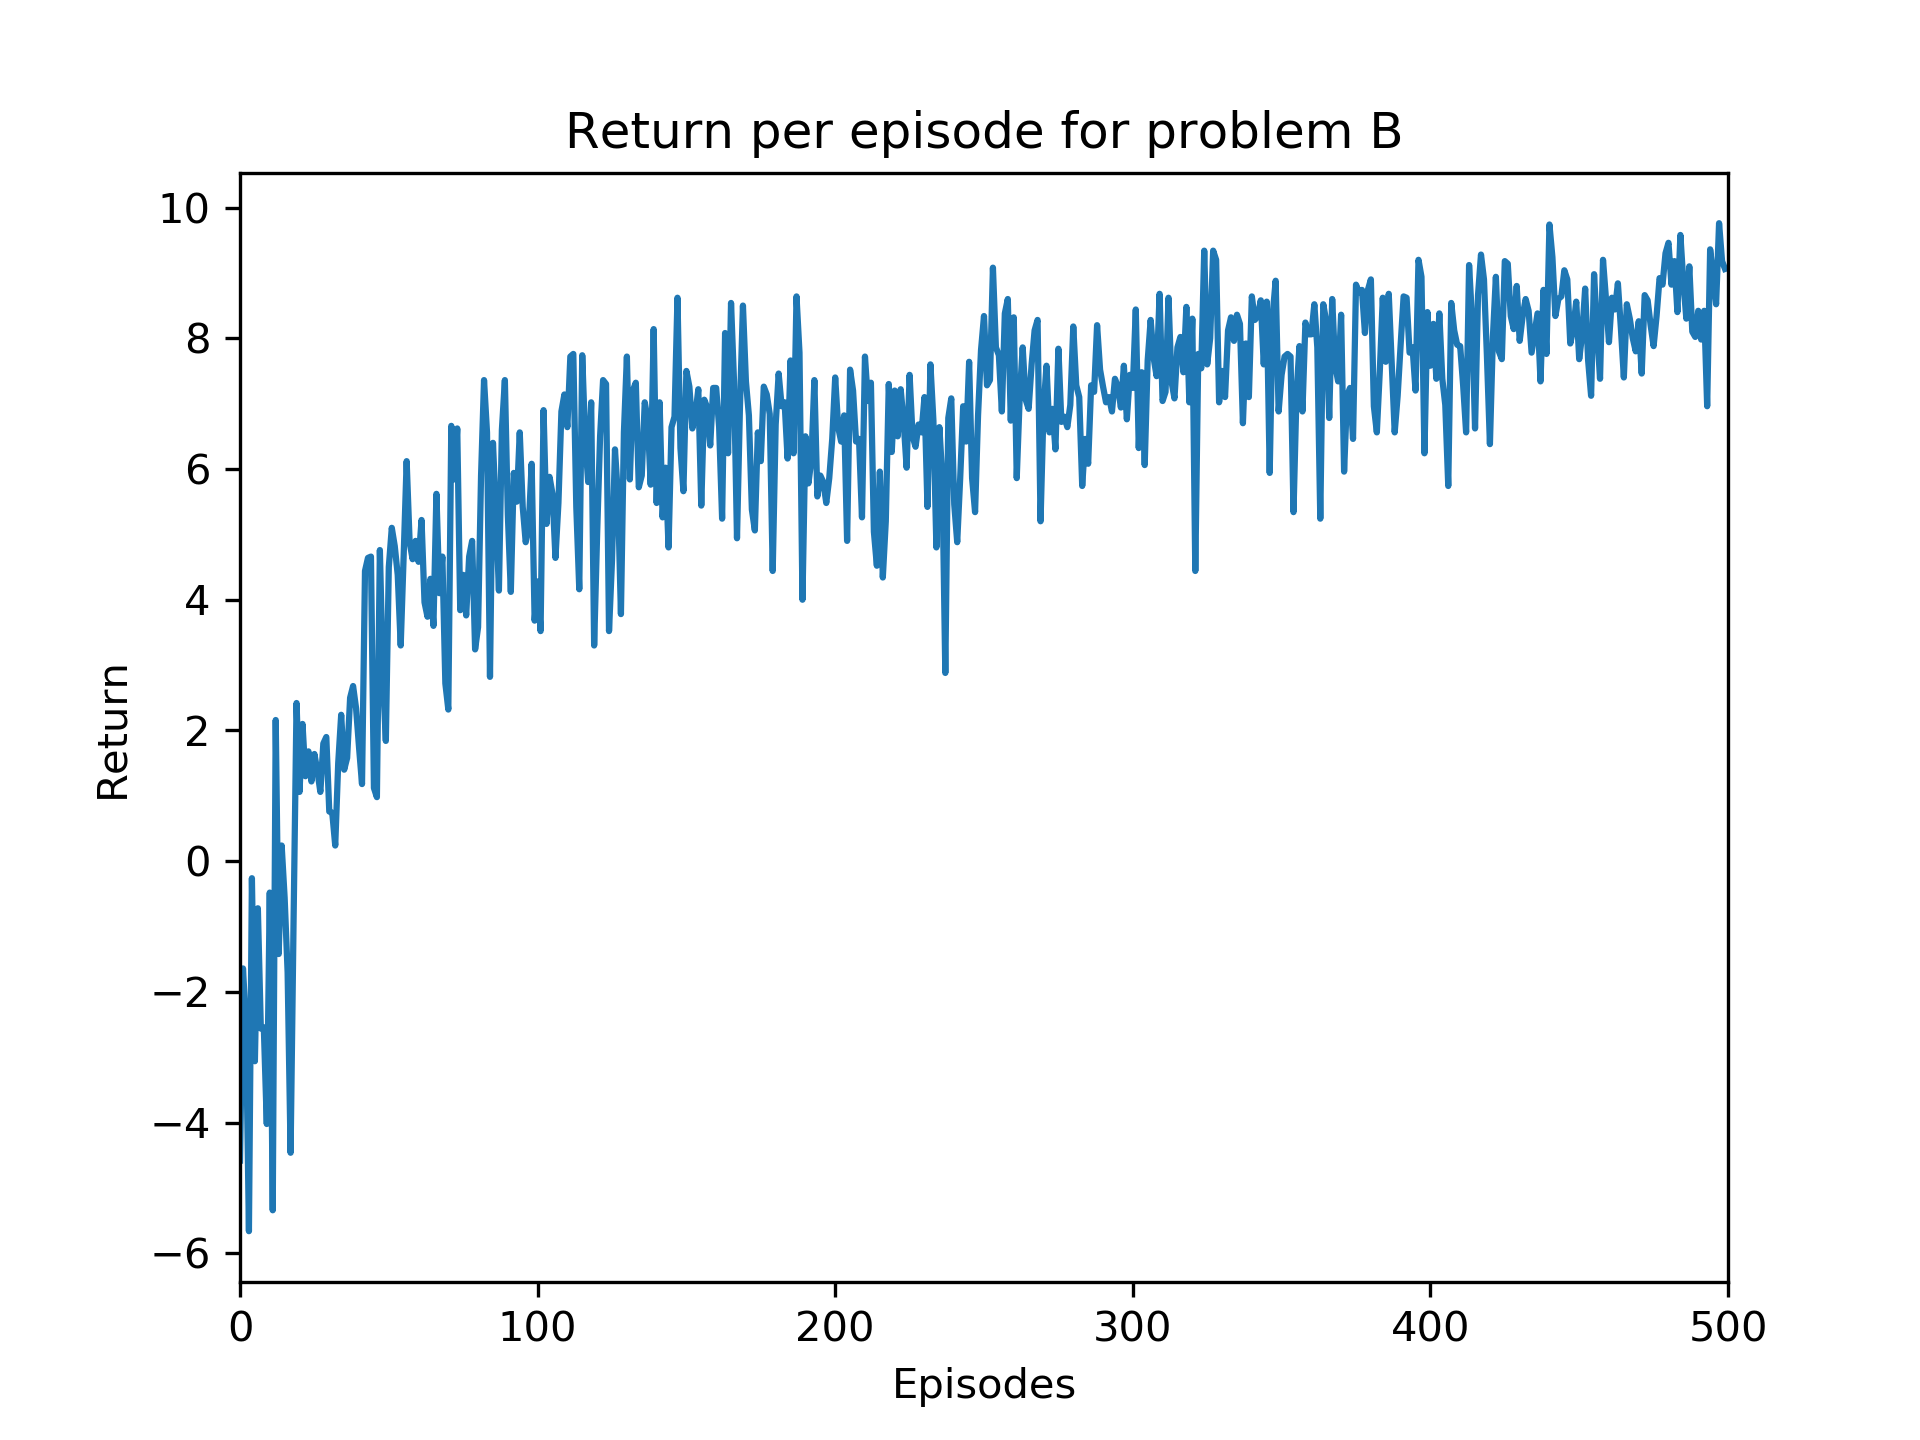
\includegraphics[width=0.4\linewidth]{./QReturn_B500.png}}
	\subfigure[Puddle World-C]
	{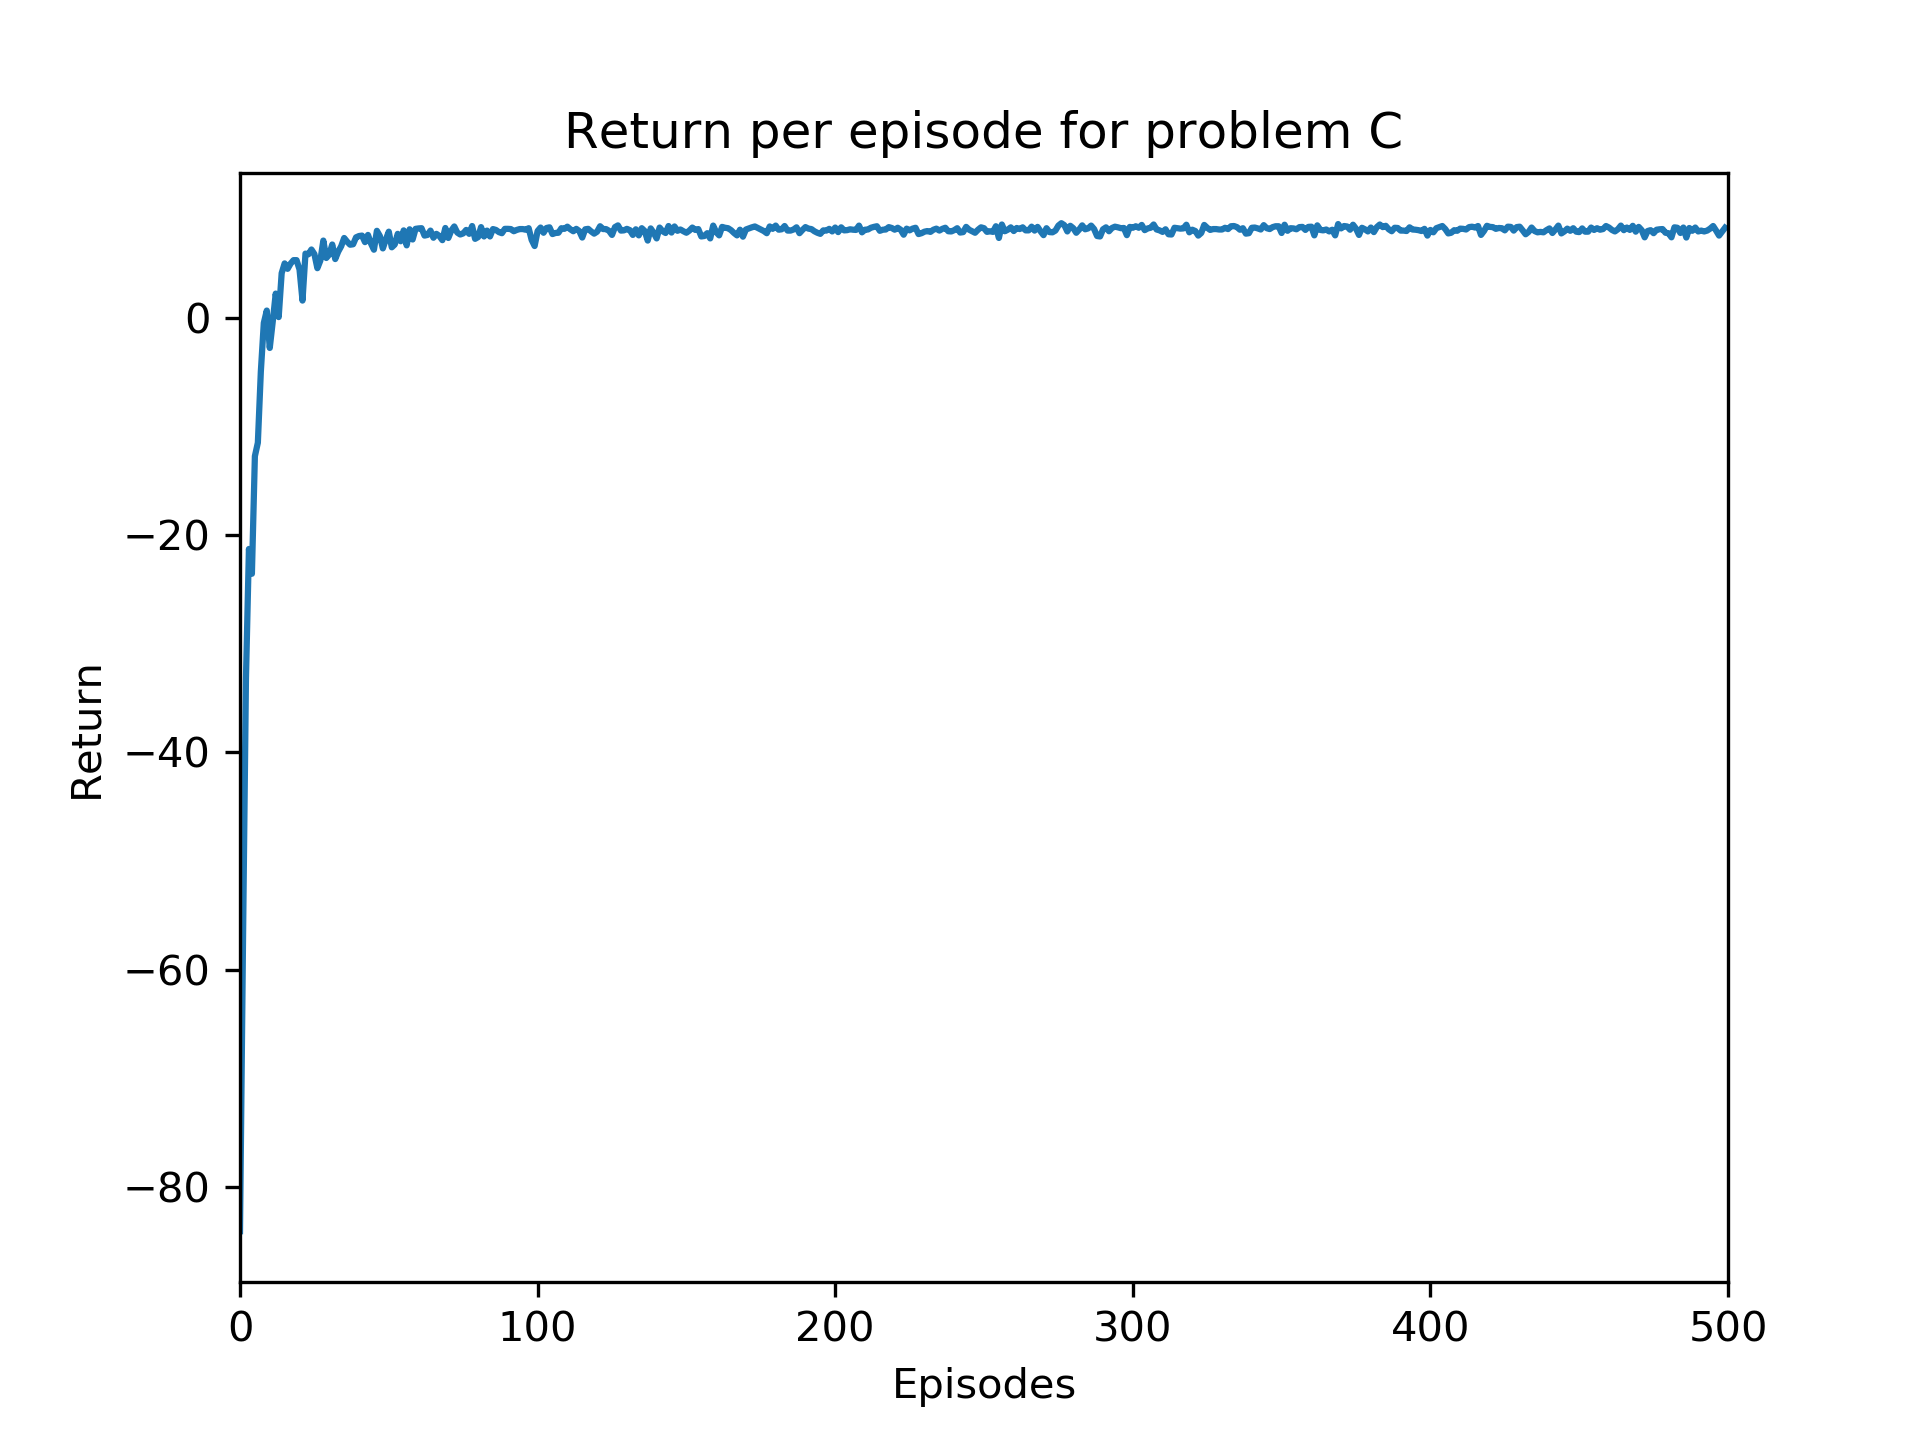
\includegraphics[width=0.4\linewidth]{./QReturn_C500.png}}
	\caption{Average return per episode obtained by the agent in different world}
	\label{fig:returnQ}
\end{figure}

From the fg:\ref{fig:combiQ}, it clear that for initial few episodes agent takes longer time to reach the goal. 
\begin{itemize}
\item 
nd{itemize}

\begin{figure}[H]
	\centering  
	\subfigure[Average steps]
	{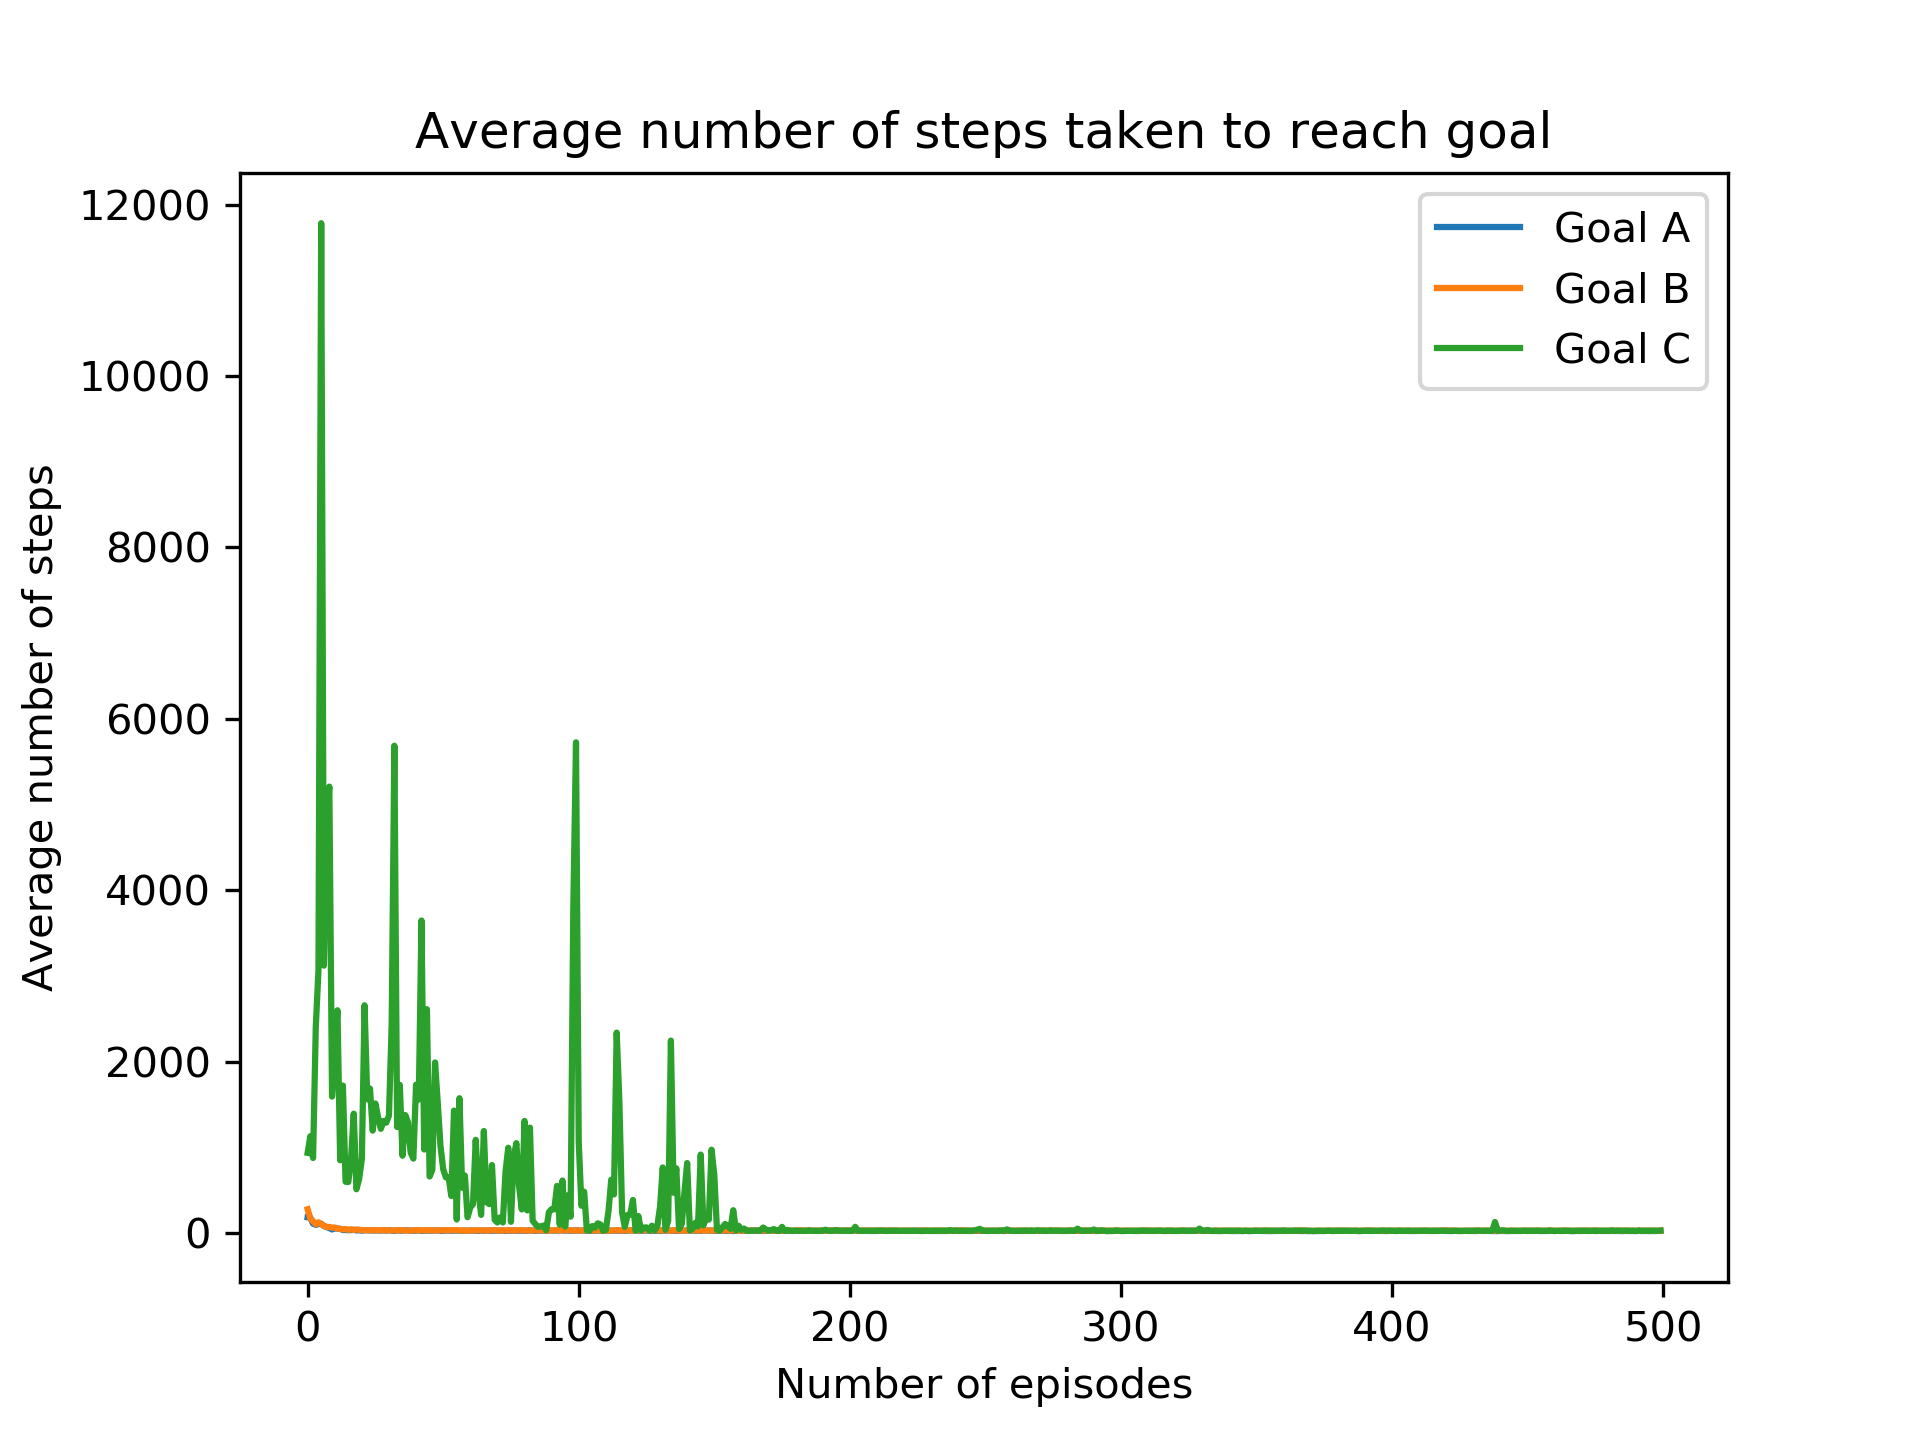
\includegraphics[width=0.4\linewidth]{./Qcombine_plot_of_avg_steps500.png}}
	\subfigure[Average return]
	{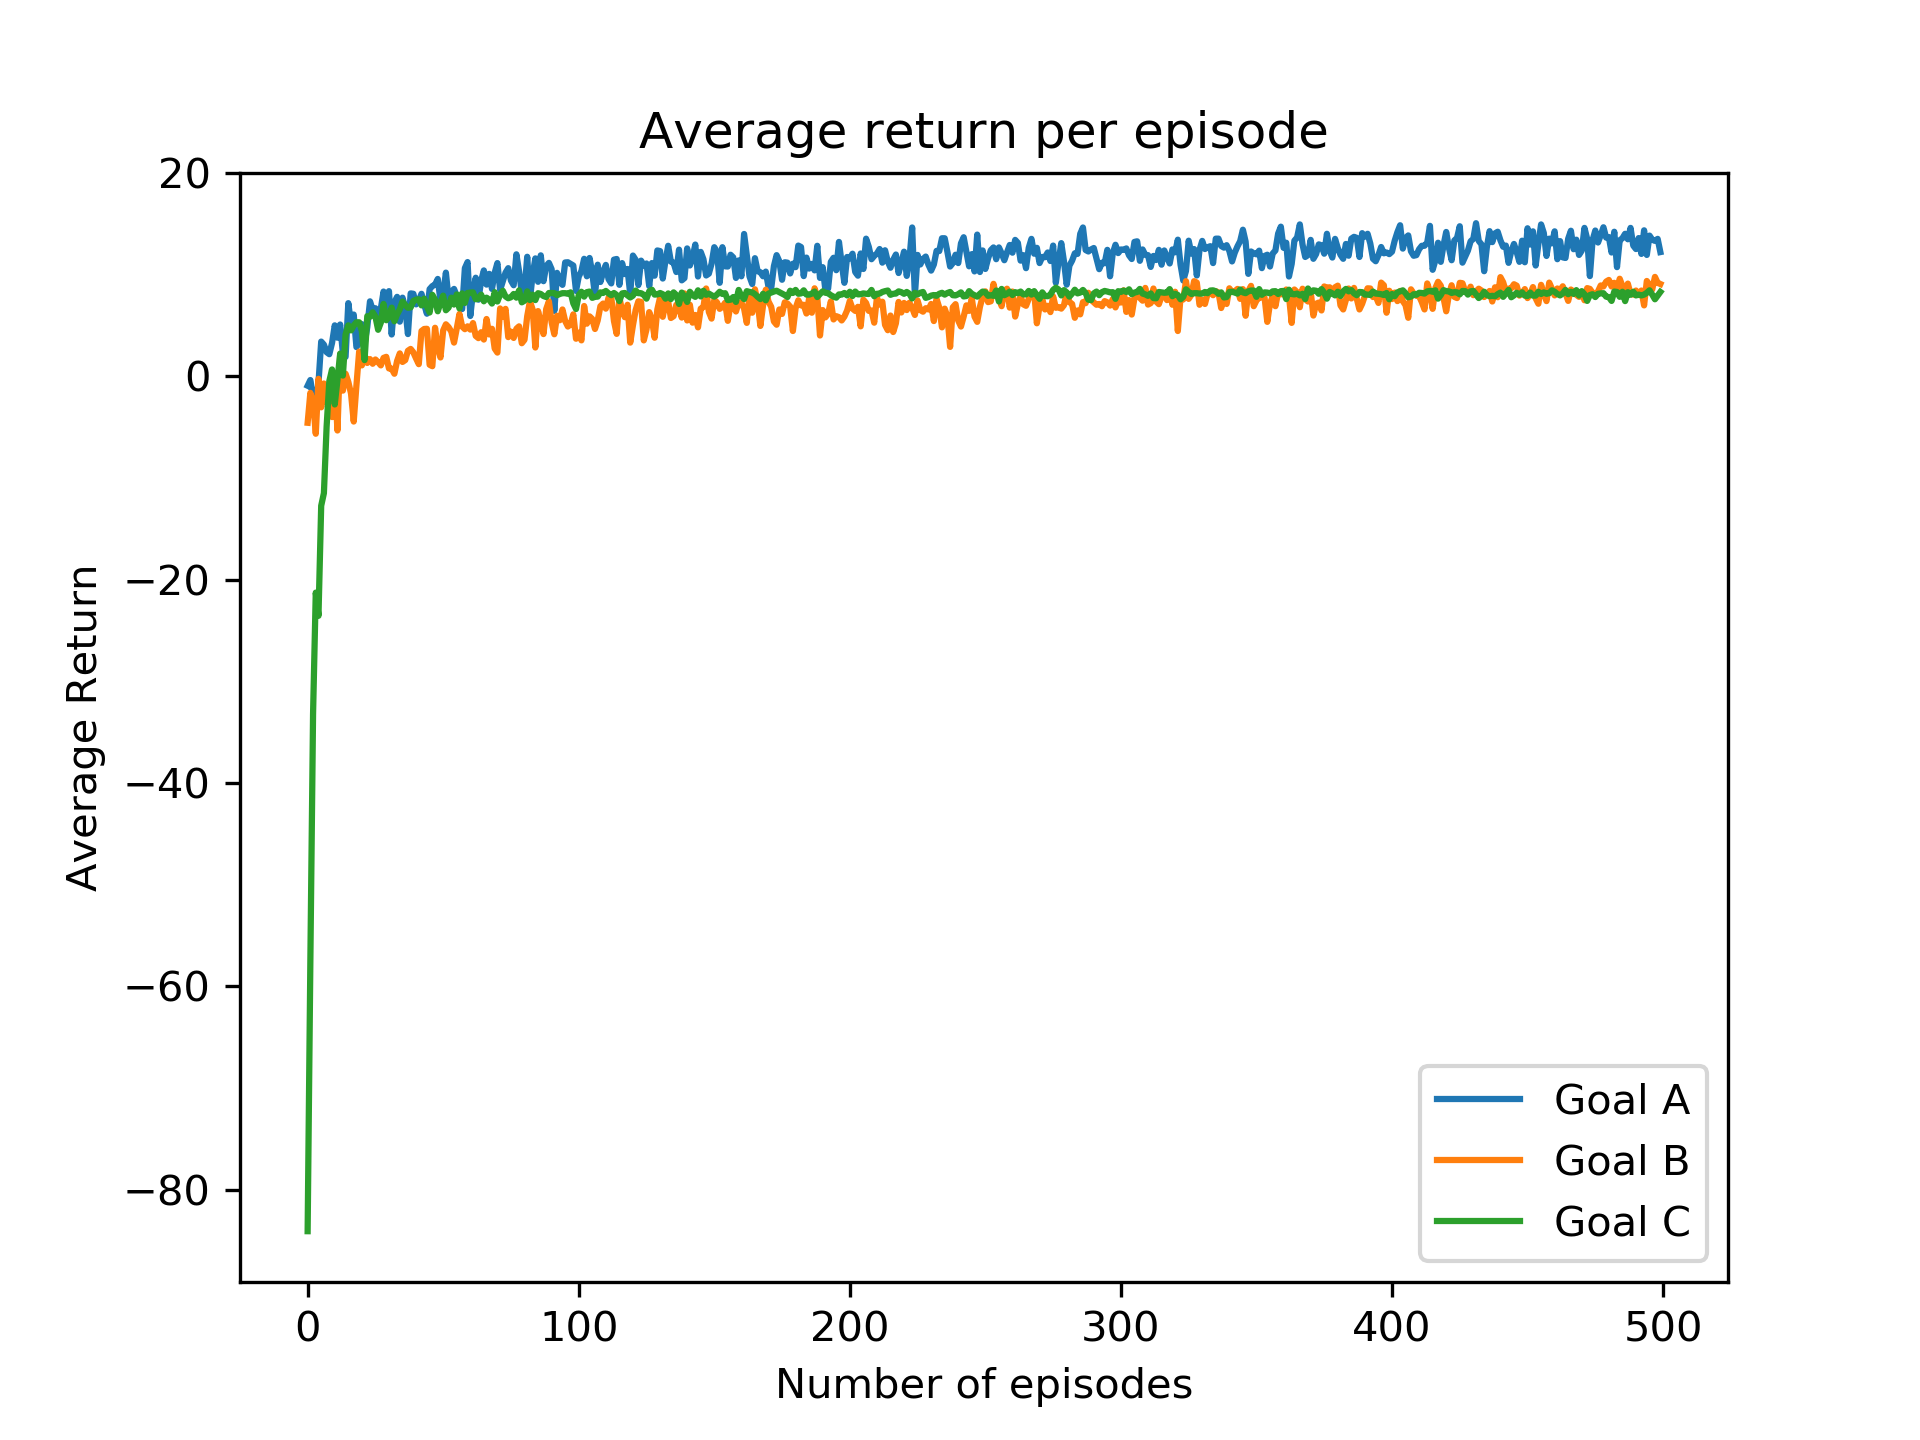
\includegraphics[width=0.4\linewidth]{./Qcombine_plot_of_avg_return500.png}}
	\caption{Combine plot of average return and average steps for different world}
	\label{fig:combiQ}
\end{figure}


\begin{figure}[H]
	\centering  
	\subfigure[Optimal Policy - A]
	{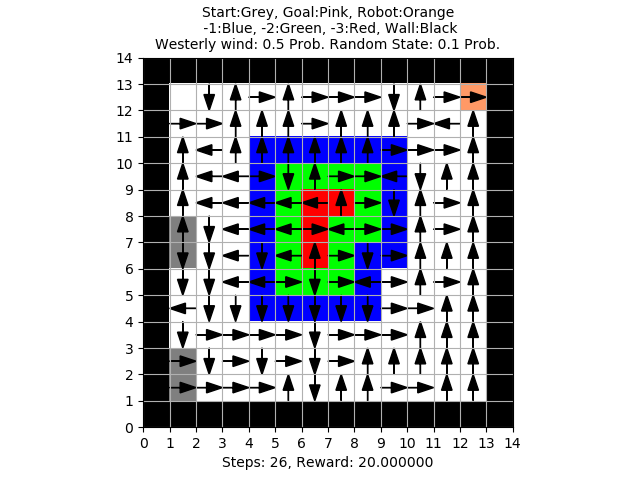
\includegraphics[width=0.4\linewidth]{./QPuddle_World_A_Arrows.png}}
	\subfigure[Optimal Policy - B]
	{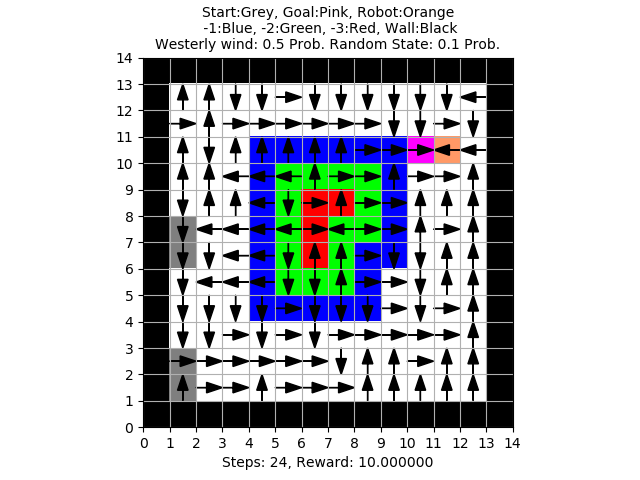
\includegraphics[width=0.4\linewidth]{./QPuddle_World_B_Arrows.png}}
	\subfigure[Optimal Policy - C]
	{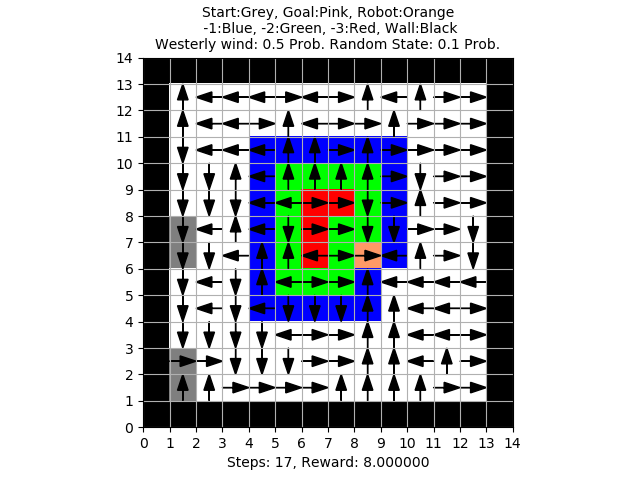
\includegraphics[width=0.4\linewidth]{./QPuddle_World_C_Arrows.png}}
	\caption{Optimal Policy obtained after learning}
	\label{fig:combiQ}
\end{figure}

%% References with bibTeX database:
\bibliographystyle{ieeetr}
\bibliography{biblio.bib}		
%%%%%%%%%%%%%%%%%%%%%%%%%%%%%%%%%%%%%%THE END%%%%%%%%%%%%%%%%%%%%%%%%%%%%%%%%%%%

\end{document}